\chapter{A brief theory of discrete time systems}
\label{chap:theory_discrete_time}

In this chapter, we consider discrete-time systems of the form
\begin{equation}\label{sys:discret}
x_{t+1}=f(x_t),
\end{equation}
with initial condition given for $t=0$ by $x_0$, with $x,x_0\in\IR^n$ and $f:\IR^n\to\IR^n$.
We also consider $p$th order equations of the form
\begin{equation}\label{eq:nth_order_discrete}
f(x_{t+p},x_{t+p-1},\dots,x_{t+1},x_t,t)=0,
\end{equation}
where $f$ is a real-valued function of the real variables $x_t$ through $x_{t+p}$ and $t$. We could also consider systems of $n$th order equations, but for the sake of brievety, we will limit ourselves to equations of the form \eqref{sys:discret} and \eqref{eq:nth_order_discrete}.

Implicit in \eqref{sys:discret} and \eqref{eq:nth_order_discrete} is that the time interval is taken to be $\Delta t=1$. Also, the state of the system at time $t$ is denoted $x_t$. Formally, \eqref{sys:discret} should be written
\[
x(t+\Delta t)=f(x(t)),
\]
but this is cumbersome and will be used only when ambiguity could lead to miscomprehensions.

Using \eqref{sys:discret}, we see that
\begin{align*}
x_1 &= f(x_0) \\
x_2 &= f(x_1)= f(f(x_0))\stackrel{\Delta}{=} f^2(x_0) \\
& \vdots \\
x_k &= f^k(x_0).
\end{align*}
The compositions
\[
f^k=\underbrace{f\circ f\circ\cdots\circ f}_{k\textrm{ times}}
\]
are called the \textbf{iterates} of $f$.
They define an infinite sequence of points
\[
x_0,x_1,x_2,\ldots,x_t,\ldots,
\]
that constitute the \textbf{solution} to \eqref{sys:discret}. The object of this chapter is to determine the behavior of this solution. For example, in the case of the logistic map \eqref{eq:logistic_map}, do solutions behave like they do for the continuous time logistic equation \eqref{eq:ODE_logistic} and tend to the carrying capacity $K$?


\section{Types of equations/systems}
% \begin{definition}
% A difference equation of order $k$ has the form $$f(x_{t+k},x_{t+k-1},\dots,x_{t+1},x_t,t)=0\quad t=0,1,\dots,$$
% where $f$ is a real-valued function of the real variable $x_t$ through $x_{t+k}$ and $t$.
% \end{definition}
\begin{definition}
The \emph{order} of a difference equation \eqref{eq:nth_order_discrete} is the difference between the largest and the smallest arguments $p$ appearing in it.
\end{definition}
Remark that in biological terms, the order $p$ of the equation is the number of previous generations that directly influence the value of $x$ in a given generation.



\begin{definition}
The difference equation is called \emph{autonomous} if $f$ does not depend explicitly on $t$ and it is called \emph{nonautonomous} otherwise.
\end{definition}



\begin{definition}
Let 
\[
x_{t+p}+a_1 x_{t+p-1}+a_2 x_{t+p-2}+\dots +a_{p-1} x_{t+1}=b_t.
\]
If the coefficients $a_j$, $j=1,\dots,p$ are constant or depend on $t$ but \textbf{do not} depend on the state variables, then the difference equation is said to be \emph{linear}; otherwise, it is \emph{nonlinear}. 
\end{definition}

\begin{definition}
If the difference equation is linear and $b_t=0$ for all $t$, then it is said to be \emph{homogeneous}; otherwise, it is said to be \emph{nonhomogeneous}.
\end{definition}



\begin{definition}
A solution of the difference equation
$$f(x_{t+k},x_{t+k-1},\dots,x_{t+1},x_t,t)=0$$
is a function $x_t$, $t=0,1,2,\dots$ such that when substituted into the equation makes it a true statement.
\end{definition}





Some characteristics of difference equations
\begin{itemize}
\item changes of states are descibed over discrete intervals. Length of the discrete interval is some fixed length $\Delta t$: states of a system are modeled at the discrete time $t=0,\Delta t, 2\Delta t, \dots$
\item recurrence relation
\item evolutionary character or not
\item to describe populations whose generations do not overlap:
\end{itemize}




\section{First-order linear difference equation}
\begin{proposition}
Consider the first-order linear homogeneous difference equation with constant coefficients
\begin{equation}\label{eq:1st_order_linearDE}
x_{t+1}=ax_t
\end{equation}
If an initial value $x_0$ is known, the solution is unique and is given by 
\begin{equation}\label{eq:sol_1storder_linear_DE}
x_t=a^tx_0.
\end{equation}
\end{proposition}

\begin{proof}
We have
\[
x_1=ax_0,
\]
and so
$$x_2=ax_1=aax_0=a^2 x_0,$$
and
$$x_3=ax_2=aaax_0=a^3x_0 \dots$$
Continuing, we have the general expression
\[
x_t=a^tx_0.\qedhere
\]
\end{proof}

Clearly, \eqref{eq:sol_1storder_linear_DE} defines a geometric sequence with common ratio $a$. Therefore, the \textbf{asymptotic behavior} of the solution depends on the value of $a$:
\begin{itemize}
\item if $|a|<1$, then $\lim_{t\rightarrow \infty}x_t=0$, i.e., $x_t$ converges to 0,
\item if $a=1$, then for all $t\geq 0$, $x_t=x_0$, i.e., $x_t$ remains constant,
\item if $a=-1$, then for all $t\geq 0$, $x_t=(-1)^tx_0$, i.e., $x_t$ alternates,
\item if $|a|>1$ then $x_t$ diverges (either approaches infinity if $a>1$ or diverges with alternating signs if $a<-1$).
\end{itemize}


\begin{proposition}
Consider the first-order linear homogeneous difference equation defined for $t=0,1,2,\dots$ by
\[
x_{t+1}=a_tx_t.
\]
If an initial value $x_0$ is known, then the solution is unique and is given by
\[
x_t=\left [\prod_{i=0}^{t-1} a_i\right ]x_0.
\]
\end{proposition}

\begin{proof}
Let us prove by mathematical induction that the proposition $P_t$ holds $\forall t\in \IN\setminus\{0\}$, with
\[
P_t: \quad x_t=\left [\prod_{i=0}^{t-1} a_i\right ]x_0.
\]
First, we consider $P_1$. We have
$$x_1=a_0x_0,$$
hence $P_1$ is true. Then assume that $P_t$ is true, i.e., $x_t=\left [\prod_{i=0}^{t-1} a_i\right ]x_0$. Now express $x_{t+1}$:
\begin{align*}
x_{t+1} &= a_tx_t \\
&=a_t\left [\prod_{i=0}^{t-1} a_i\right ]\;x_0 \quad\textrm{(by induction hypothesis)}\\
&= \left [\prod_{i=0}^t a_i\right ]x_0,
\end{align*}
so $P_{t+1}$ is true.
By the principle of mathematical induction (PMI), we conclude that 
\[
x_t=\left [\prod_{i=0}^{t-1} a(i)\right ]x_0, \forall t\in \IN\setminus\{0\}.\qedhere
\]
\end{proof}


\begin{proposition}\label{Prop:FirstLinNonH}
Consider the first-order linear nonhomogeneous difference equation defined for $t=0,1,2,\dots$ by
$$x_{t+1}=a_tx_t + b_t.$$
If an initial value $x_0$ is known, then the solution is unique and is given by
\[
x_t=\left [\prod_{i=0}^{t-1} a_i\right ]x_0 +b_{t-1}+\sum_{i=0}^{t-2}\left [ \prod_{r=i+1}^{t-1} a_r \right]b_i.
\]
In particular,
\begin{itemize}
\item If $x_{t+1}=a x_t + b_t$, then 
$$x_t=a ^t x_0 +\sum_{i=0}^{t-1} a^{t-i-1}b(i).$$
\item If $x_{t+1}=a x_t + b$, then 
$$x_t=
\begin{cases}
a ^t x_0 +b\left[\dfrac{a^t-1}{a-1}\right] & a\not =1\\  
x_0 +bt & a =1.
\end{cases}
$$
\end{itemize}
\end{proposition}


\begin{proof}
Let us prove by mathematical induction that
\[
P_t:\quad
x_t=\left [\prod_{i=0}^{t-1} a_i\right ]x_0 +b_{t-1}+\sum_{i=0}^{t-2}\left [ \prod_{r=i+1}^{t-1} a_r \right]b_i
\]
holds true for all $t\in \IN\setminus\{0\}$.
At rank $t=2$: $x_1=a_0x_0+b_0$, then
$$x_2=a_1x_1+b_1=a_1a_0x_0+a_1b_0+b_1.$$
%Similarly for $x_3$
%$$x_3=a(2)x_2+b(2)=a(2)a(1)a(0)x_0+a(2)a(1)b(0)+a(2)b(1)+b(2)$$
Now assume that $P_t$ holds true, i.e., 
$$x_t=\left [\prod_{i=0}^{t-1} a_i\right ]x_0 +b_{t-1}+\sum_{i=0}^{t-2}\left [ \prod_{r=i+1}^{t-1} a_r \right]b_i$$
and express $x_{t+1}$:
\begin{align*}
x_{t+1} &= a_tx_t+b_t \\
&=a_t\left\{\left[\prod_{i=0}^{t-1} a_i\right]x_0 +b_{t-1}
+\sum_{i=0}^{t-2}\left[\prod_{r=i+1}^{t-1} a_r \right]b_i \right\}+b_t \\
&=\left[a_t\prod_{i=0}^{t-1} a_i\right ]x_0+a_tb_{t-1}+\sum_{i=0}^{t-2}\left [ a_t\prod_{r=i+1}^{t-1} a_r \right]b_i+b_t \\
&=\left [\prod_{i=0}^{t} a_i\right ]x_0+b_t+a_tb_{t-1}+\sum_{i=0}^{t-2}\left [ \prod_{r=i+1}^{t} a_r \right]b_i \\
&= \left [\prod_{i=0}^{t} a_i\right ]x_0+b_t
+\sum_{i=0}^{t-1}\left [ \prod_{r=i+1}^{t} a_r \right]b_i.
\end{align*}
Thus $P_{t+1}$ holds.
By the principle of mathematical induction, we conclude that, for all $t\in\IN\setminus\{0\}$, 
$$x_t=\left [\prod_{i=0}^{t-1} a_i\right ]x_0 +b_{t-1}+\sum_{i=0}^{t-2}\left [ \prod_{r=i+1}^{t-1} a_r \right]b_i.\qedhere$$
\end{proof}

\section{Higher-order linear equations}
\begin{definition}
The functions $x_t^1$, $x_t^2$,$\dots, x_t^k$ are said to be linearly independent for $t\geq t_0$ whenever 
$$a_1x^1_t+a_2x^2_t+\dots + a_kx^k_t=0$$
for all $t\geq t_0$, then we must have $a_1=a_2= \dots =a_k=0$.
\end{definition}

\begin{definition}
The Casoratian of $k$ functions $x_t^1$, $x_t^2$,$\dots, x_t^k$ is
$$C(x_t^1, x_t^2,\dots, x_t^k)=\det \left (
\begin{array}{cccc}
x_t^1 & x_t^2 & \dots & x_t^k\\
x_{t+1}^1 & x_{t+1}^2 & \dots & x_{t+1}^k\\
x_{t+2}^1 & x_{t+2}^2 & \dots & x_{t+2}^k\\
\vdots & & &\\
x_{t+k-1}^1 & x_{t+k-1}^2 & \dots & x_{t+k-1}^k\\
\end{array}\right )$$
\end{definition}

\begin{proposition}
If the Casoratian of $x_t^1$, $x_t^2$,$\dots, x_t^k$ satifies
$$C(x_t^1, x_t^2,\dots, x_t^k)\not =0 \quad \forall t$$
then $x_t^1$, $x_t^2$,$\dots, x_t^k$  are $k$ linearly independent functions.
\end{proposition}

\begin{definition}
A set of $k$ linearly independent solutions of a $k^{th}$ linear homogeneous difference equation is called a fundamental set of solutions.
\end{definition}

\begin{proposition}(Principle of superposition)
If $x_t^1$, $x_t^2$,$\dots, x_t^k$ are solutions a $k^{th}$ linear homogeneous difference equation then $$c_1x_t^1+c_2x_t^2+\dots, c_kx_t^k$$
is also solution of the $k^{th}$ linear homogeneous difference equation.
\end{proposition}

\begin{definition}
Let $\{x_t^1, x_t^2,\dots, x_t^k\}$ be a fundamental set of solutions of $k^{th}$ linear homogeneous difference equation. Then the general solution of the  $k^{th}$ linear homogeneous difference equation is given by $$x_t=\sum_{i=1}^kc_ix^i_t,$$ for arbitrary constants $c_i$, $i=1,\dots, k$
\end{definition}

\subsection[Homogeneous autonomous higher-order linear equations]{Homogeneous equations with constant coefficients}
The case of a second-order equation is derived to illustrate this subsection.

A second-order linear homogeneous equation with constant coefficients:
\begin{equation}\label{eq:SecLinHom}
a_0x_{t+2}+a_1x_{t+1}+ a_2 x_{t}=0
\end{equation}
To find two linearly independent solutions, $x_t^1$ and $x_t^2$: assume that solutions take the form of 
$x_t=\lambda ^t$ with $\lambda \not= 0$. Then substitute solution in \eqref{eq:SecLinHom}
$$a_0\lambda ^{t+2}+a_1\lambda ^{t+1}+ a_2 \lambda ^{t}=0,$$
$$a_0\lambda ^{2}+a_1\lambda + a_2 =0.$$

The equation $a_0\lambda ^{2}+a_1\lambda + a_2 =0$ is the \textbf{characteristic equation} of \eqref{eq:SecLinHom}. The 2 roots of the characteristic equation, $\lambda_1$ and $\lambda_2$, are the \textbf{eigenvalues}.

The general solution is a linear combination of the 2 solutions $x_t^1=\lambda_1^t$ and $x_t^2=\lambda_2^t$. The form of the general solution depends on the eigenvalues and there are 3 cases:
\begin{description}
\item[Eigenvalues are real and distinct:] $\lambda _1 \not = \lambda _2 $. The general solution is
$$x_t=c_1\lambda _1 ^t+c_2\lambda _2 ^t,$$
with $c_1$ and $c_2$ arbitrary constants.
\item[Eigenvalues are real and equal:] $\lambda _1  = \lambda _2 $. Then the $2$ linearly independent solutions are  $x_t^1=\lambda _1^t$ $x_t^2=t\lambda _2^t$. 
The general solution is
$$x_t=c_1\lambda _1 ^t+c_2t\lambda _2 ^t,$$
with $c_1$ and $c_2$ arbitrary constants.
\item[Eigenvalues are complex conjugates:] $\lambda _{1,2}=A\pm iB=r(\cos \phi \pm i \sin \phi)$, where $r=\sqrt{A^2+B^2}$ and $\phi=\arctan(B/A)$. The two linearly independent solutions are $x^1=r^t\cos(t\phi)$ and $x^2=r^t\sin (t\phi)$.
Then the general solution is
$$x_t=c_1 r^t\cos(t\phi)+c_2r^t\sin (t\phi),$$
with $c_1$ and $c_2$ arbitrary constants.
\begin{center}
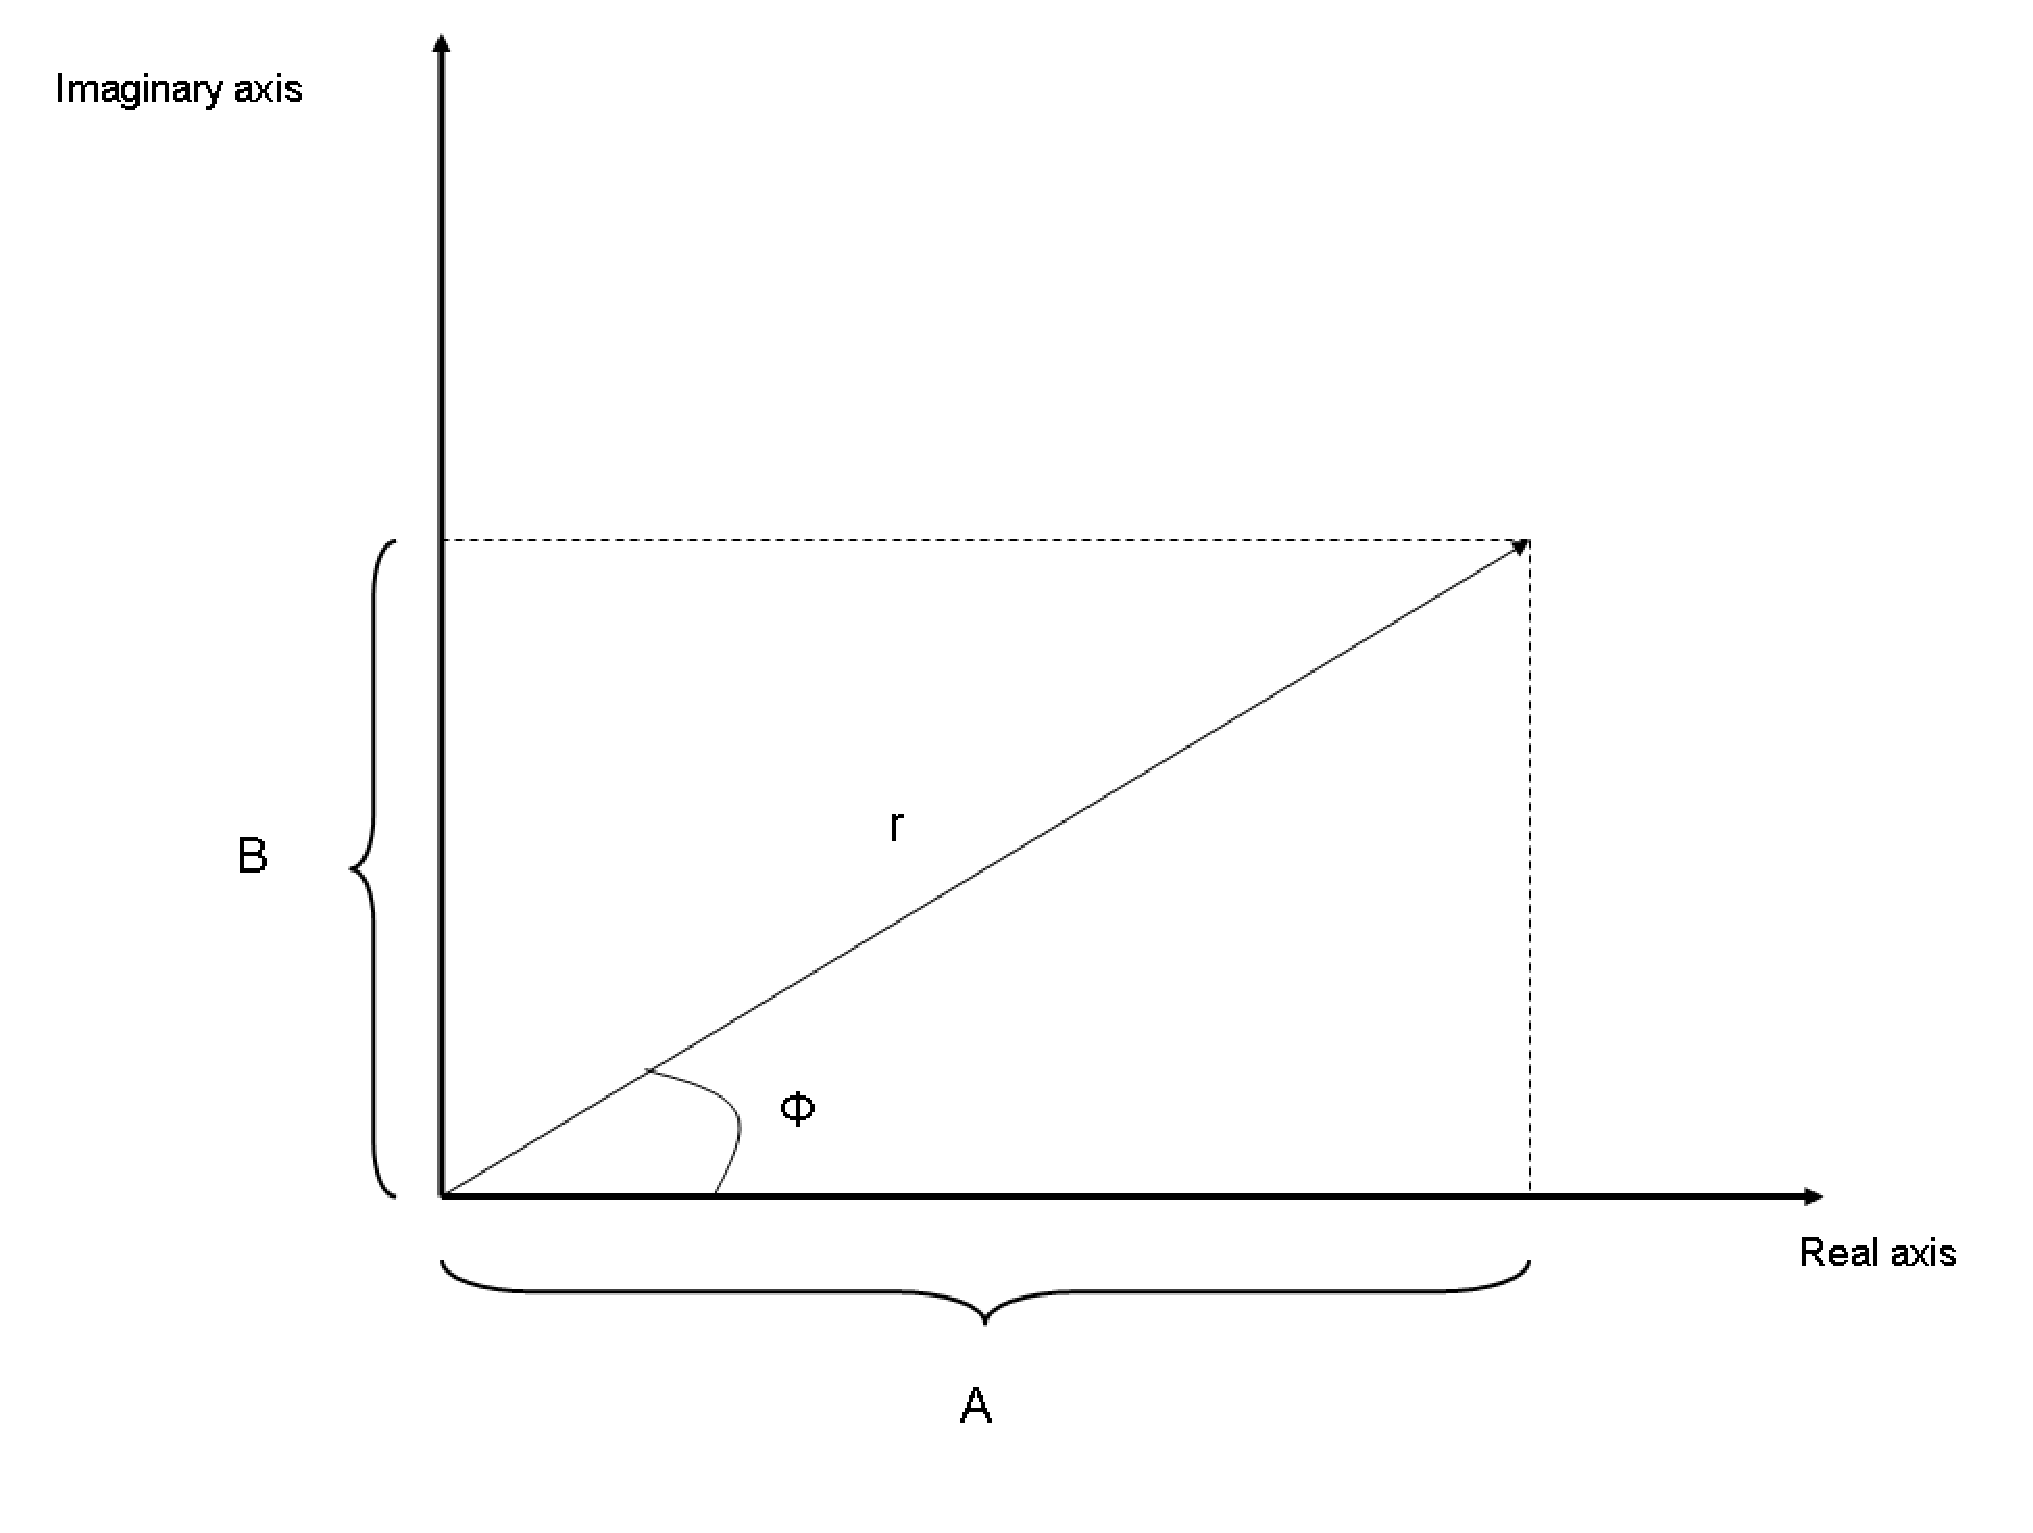
\includegraphics[width=.5\textwidth]{figs_steph/FigurePhase}
\end{center}
\end{description}


An $m^{th}-$order linear homogeneous equation with constant coefficients is defined as
\begin{equation}\label{eq:LinH}
a_0x_{t+m}+a_1x_{t+m-1}+\dots + a_m x_{t}=0
\end{equation}
Solutions are composed of linear superpositions of $m$ solutions of the form 
$x_t=\lambda ^t$, $\lambda \not = 0$
where $\lambda$ are obtained by finding the roots (eigenvalues) of the characteristic equation
$$a_0\lambda^{m}+a_1\lambda^{m-1}+\dots + a_m =0.$$
The characteristic equation has $m$ eigenvalues: $\lambda _i,$ $i=1,\dots, m$. 

If eigenvalues are all real and distinct, the general solution takes the form
$$x_t=c_1\lambda_1^t+\dots +c_m\lambda_m^t$$
where $c_i$, $i=1,\dots ,m$ are arbitrary.

For the other cases, general solutions depend on the existence of repeated or complex conjugate eigenvalues. If there is a real eigenvalue $\lambda _1$ of multiplicity $k$, then $k$ linearly independent solutions can be formed by multiplying by powers of $t$:
$$\lambda_1 ^t, t \lambda_1 ^t, t^2\lambda_1 ^t, \dots , t^{k-1}\lambda_1 ^t.$$
If there are complex eigenvalues $\lambda _{1,2}=r(\cos \phi \pm i \sin \phi)$ of multiplicty $k$, then there are $2k$ linearly independent solutions:
$$r^t\cos(t\phi),r^t\sin (t\phi),tr^t\cos(t\phi),tr^t\sin (t\phi),\dots,t^{k-1}r^t\cos(t\phi),t^{k-1}r^t\sin (t\phi)$$




\subsection{Nonhomogeneous equations}
An $m^{th}-$order linear nonhomogeneous equation  is defined as
\begin{equation}\label{eq:LinNonH}
a_0x_{t+m}+a_1x_{t+m-1}+\dots + a_m x_{t}=b(t)
\end{equation}

\begin{theorem}
The general solution of \eqref{eq:LinNonH} is
$$x_t=x_t^p+\sum_{i=1}^m a_i x_t^i$$
where $x_t^p$ is a particular solution of the nonhomogeneous equation and $\{x_t^1, x_t^2,\dots, x_t^k\}$ is a fundamental set of solutions of $m^{th}$ homogeneous equation \eqref{eq:LinH}.
\end{theorem}


To find a particular solution of a nonhomogeneous equation, there exist several methods:
\begin{description}
\item[Method of undetermined coefficient:] making a guess as to the form of the particular solution, and then substituting this function in the difference equation. This method works if the nonhomogeneous term $b(t)$ is a linear combination or product of terms having one of the forms
$$a^t, \quad \cos(ct), \quad  \sin(ct), \quad t^k.$$
See Table \ref{Table1}.
\item[Method of variation of constants]
\end{description}

\begin{table}
\begin{center}
\begin{tabular}{c|p{7cm}}
$b(t)$ & \multicolumn{1}{c}{$x_t^p$}
\\\hline
$a^t$ & $c_1 a^t$\\
$t^k$ & $c_0+c_1t+c_2t^2+\dots+c_k t^k$\\
$t^ka^t$ & $c_0a^t+c_1ta^t+c_2t^2a^t+\dots+c_k t^ka^t$\\
$\sin(ct),\cos(ct)$ & $c_1\sin(ct)+c_2\cos(ct)$\\
$a^t\sin(ct),a^t\cos(ct)$ & $(c_1\sin(ct)+c_2\cos(ct))a^t$\\
$a^tt^k\sin(ct),a^tt^k\cos(ct)$ & $(d_0+d_1t+d_2t^2+\dots+d_k t^k)\sin(ct)a^t+(c_0+c_1t+c_2t^2+\dots+c_k t^k)\cos(ct)a^t$\\
\end{tabular}
\label{Table1}
\caption{Particular solutions}
\end{center}
\end{table}


\subsection{Qualitative analysis}
What is the long-term behaviour of the solutions?

For linear difference equations, the asymptotic behavior depends on the eigenvalues: real and complex and the magnitude of eigenvalues.

\begin{definition}
Magnitude of an eigenvalue:
\begin{itemize}
\item If $\lambda=A$ is real, $|\lambda|=|A|$.
\item If $\lambda=A+iB$ is complex, $|\lambda|=|A+iB|=\sqrt{A^2+B^2}$.
\end{itemize}
\end{definition}


\begin{definition}
An eigenvalue $\lambda _i$ such that
$$|\lambda _i|\geq |\lambda _j|$$
for all $j\not =i$ is called the dominant eigenvalue. If the inequality is strict, then $\lambda _i$ is a strictly dominant eigenvalue.
\end{definition}

%\begin{itemize}
%\end{itemize}

Let the general solution of \eqref{eq:LinH} be
$$x_t=\sum_{i=1}^m c_i \lambda_i^t$$

The limiting behavior of the general solution is determined by the behavior of the dominant solution (correspondant to the dominant eigenvalue). Let $\lambda _1$ be the strictly dominant eigenvalue ($|\lambda _1|> |\lambda _j|$ for all $j\not =1$) then
$$x_t=\lambda _1^t\left[ c_1+\sum_{i=2}^m c_i\left ( \frac{\lambda_i}{\lambda_1}\right )^t\right ]$$
Since $\left |\frac{\lambda _i}{\lambda _1}\right |<1$, for all $i\not =1$, then $\left ( \frac{\lambda_i}{\lambda_1}\right )^t\rightarrow 0$ as $t\rightarrow +\infty$. Then $$\lim _{t\rightarrow +\infty }x_t=\lim _{t\rightarrow +\infty }c_1\lambda _1^t.$$
Depending on the value of $\lambda _1$ there are different situations
\begin{itemize}
\item $\lambda _1$ Real
\begin{itemize}
\item $\lambda _1 >1:$ $\lim _{t\rightarrow +\infty }c_1\lambda _1^t=\infty$ (monotonically diverge $\Rightarrow$ unstable system)
\item $\lambda _1 =1:$ constant
\item $0 <\lambda _1 <1:$ $\lim _{t\rightarrow +\infty }c_1\lambda _1^t=0$ (monotonically decreasing to 0 $\Rightarrow$ stable system)
\item $-1 <\lambda _1 <0:$ $\lim _{t\rightarrow +\infty }c_1\lambda _1^t=0$ (oscillating around zero and converging to 0 $\Rightarrow$ stable system)
\item $\lambda _1 =-1:$ system oscillating between two values $c_1$ and $-c_1$
\item $\lambda _1 <-1:$ system is oscillating but increasing in magnitude (unstable system)
\end{itemize}
\item $\lambda _1$ Complex
\begin{itemize}
\item $|\lambda _1|>1$: system oscillates but increases in magnitude (unstable system)
\item $|\lambda _1|=1$: system oscillates but constant magnitude 
\item $|\lambda _1|<1$: system oscillates but converges to 0 (stable system)
\end{itemize}
\end{itemize}

Magnitude of eigenvalues determine whether solutions are unbounded or bounded. The nature, real or complex determine whether solutions oscillate, or not.

In the case of a nonhomogeneous difference equation with a constant nonhomogeneous term, if the system converges, it will converge to the equilibrium point $x^*$ (not to $0$ as previously).



\section{First-order linear systems}
A higher-order linear difference equation can be converted to a first-order linear system.
Consider the $m^{th}$-order linear nonhomogeneous equation 
\[
a_0x_{t+m}+a_1x_{t+m-1}+\dots + a_m x_{t}=b(t).
\]
For convenience $x_t$ is now denoted $x(t)$. Let $Y(t)$ be a $m$-vector  $Y(t)=(y_1(t),y_2(t),\dots, y_m(t))$ that satisfies
\begin{align*}
y_1(t)&=x(t)\\
y_2(t)&=x(t+1)\\
y_3(t)&=x(t+2)\\
\vdots& \\
y_{m}(t)&=x(t+m-1).
\end{align*}
The first element $y_1(t)$ is the solution $x(t)$. Hence a first-order difference equation in $y$ is 
\begin{align*}
y_1(t+1)&=y_2(t)\\
y_2(t+1)&=y_3(t)\\
y_3(t+1)&=y_4(t)\\
\vdots &\\
y_{m-1}(t+1)&=y_{m}(t)\\
y_{m}(t+1)&=-a_1 y_m(t)-\dots -a_{m-1}y_2(t)- a_m y_1(t)+b(t)
\end{align*}
In matrix form,
$$Y(t+1)=AY(t)+B$$
where
$$A=\left (
\begin{array}{ccccc}
0 & 1 & 0 & \hdots & 0\\
0 & 0 & 1 & \hdots & 0\\
\vdots & \vdots & \vdots & \ddots & \vdots\\
0 & 0 & 0 & \hdots & 1\\
-a_{m} & -a_{m-1} & -a_{m-2} & \hdots & -a_{1}
\end{array}
\right), \quad B=\left ( \begin{array}{c}
0\\
0\\
\vdots\\
0\\
b(t)
\end{array}
\right).
$$ 
The matrix $A$ has 1's along the superdiagonal and has the coefficients of the higher-order difference equation $-a_i$ (but the signs are reversed) along the last row. Matrix is called the {\bf companion matrix} of the $m^{th}-$order difference equation.


A solution to a first-order linear difference system $X(t+1)=AX(t)+B$ is the superposition of two solutions: the general solution $X_h$ to the homogeneous system $X_h(t+1)=AX_h(t)$ and a particular solution $X_p$ to the nonhomogeneous system $X_p(t+1)=AX_p(t)+B$. The general solution to the nonhomogeneous system is $$X(t)=X_h(t)+X_p(t).$$


The homogeneous system has $m-$linearly independent solutions: there are some direct and indirect methods to find these linearly independent solutions.

{\bf Indirect methods} use the fact that the solution can be expressed as $X(t)=A^tX(0). $ In \cite{Elaydi1998}, methods to compute $A^t$ are presented, then the general solution can be known.

{\bf Direct method} to solve $X(t+1)=AX(t)$ where $A=(a_{ij})$ is an $m\times m$ constant matrix:
Assume that a solution has the following form $X(t)=\lambda ^t V$ where $V$ is an nonzero $m-$column vector and $\lambda$ is a constant. Substituting $\lambda ^t V$ into the linear system gives
$$\lambda ^{t+1} V=A\lambda ^t V,$$
then
\begin{equation}(A - \lambda I) V=\mathbf{0}\label{eq:Cha}\end{equation}
where $I$ is the $m\times m$ identity matrix and $\mathbf{0}$ is the zero vector. The zero solution $V=0$ is the trivial solution; and \eqref{eq:Cha} has an unique solution if $\det(A - \lambda I)\not =0$. Hence, nonzero solutions $V$ are obtained if and only if $(A - \lambda I) $ is singular if and only if 
\begin{equation}\det(A - \lambda I) =0.\label{eq:Charac}\end{equation}

Equation \eqref{eq:Charac} is referred as the {\bf characteristic equation of matrix} $A$. The $m$ solutions $\lambda_i$, $i=1,\dots, m$ of \eqref{eq:Charac} are called the {\bf eigenvalues} of the matrix $A$. The nonzero solutions $V_i$ are the {\bf eigenvectors} corresponding to the eigenvalue $\lambda_i$ that are found by solving $(A - \lambda_i I) V_i=\mathbf{0}$.

Then the general solution is a linear combination of $m$ linearly independent solutions $X_i=\lambda _i ^t V_i$, $i=1,\dots, m$:
\begin{equation}X(t)=\sum_{i=1}^m c_i\lambda _i ^t V_i\label{eq:solFirstSyst}\end{equation}
where $c_i$ are arbitrary constants.

The asymptotic behavior of the solution \eqref{eq:solFirstSyst} does not require the knowlegde of the eigenvectors. The asymptotic behavior is determined by the eigenvalues and their magnitude.

\begin{definition}
The spectral radius of matrix $A$ is denoted $\rho(A)$ and is defined as
$$\rho(A)=\max_{i\in \{1,2,\dots,m\}}|\lambda_i|$$
\end{definition}


\begin{theorem}\label{Theo:NormRho}
Let $A$ be a $k\times k$ matrix
$$\rho(A)\leq \| A\| $$
\end{theorem}

Three usual matrix norms are
\begin{itemize}
\item $ \| A\|_1=\max_{1\leq j\leq k}\sum_{i=1}^k|a_{ij}|$ (sum over columns),
\item $ \|A\|_2=[\rho(A^TA)]^{1/2}$
\item $\|A\|_{\infty}=\max_{1\leq i\leq k}\sum_{j=1}^k|a_{ij}|$ (sum over rows).
\end{itemize}








\begin{theorem}\label{Theorem:MatrixConverg}
Let $A$ be a constant $m \times m$ matrix. Then the spectral radius of $A$ satisfies $\rho(A)<1$ if and only if $$\lim_{t\rightarrow + \infty}A^t=\mathbf{0}$$
\end{theorem}

As the solution of $X(t+1)=AX(t)$ is $X(t)=A^tX(0)$, $\lim_{t\rightarrow + \infty} X(t)=0$ when $\rho(A)<1$.

\subsection{Nonnegative matrices}
\begin{definition}
A matrix $A$ whose entries are nonnegative is called a nonnegative matrix, denoted $A\geq 0$.
\end{definition}


\begin{definition}
A matrix $A$ whose entries are positive is called a positive matrix, denoted $A> 0$.
\end{definition}


\begin{definition}
A square $m\times m$  matrix $A=a_{ij}$ is \textbf{reducible} if the index set $1,2, \dots, m$ can be split into two nonempty complementary sets $S_1$ and $S_2$: $S_1=\{i_1,\dots , i_{\mu}\}$ and $S_2=\{k_1,\dots , k_{\varepsilon}\}$ where $m=\mu+\varepsilon$ such that
$$a_{i_\alpha k_{\beta}}=0 \quad (\alpha = 1,2,\dots , \mu; \beta = 1,2, \dots, \varepsilon).$$
Otherwise, the matrix $A$ is \textbf{irreducible}.
\end{definition}


\begin{definition}
If there exits a directed path from node $i$ to $j$ for every node $i$ and $j$ in the digraph, then the digraph is said to be strongly connected.
\end{definition}

\begin{theorem}
The digraph of matrix $A$ is strongly connected if and only if $A$ is irreductible.
\end{theorem}


\begin{theorem}(Frobenius Theorem)
An irreductible, nonnegative matrix $A$ always has a positive eigenvalues $\lambda$ that is a simple root (multiplicity one) of the characteristic equation. The value of $\lambda$ is greater than or equal to the magnitude of all of the other eigenvalues. To the eignevalue $\lambda$ there corresponds an eigenvector with positive coordinates.
\end{theorem}


\begin{theorem}(Perron Theorem)
A positive matrix $A$ always has a real, positive eigenvalue $\lambda$ that is a simple root of the characteristic equation and exceeds the magnitude of all of the other eigenvalues
$$|\lambda _i|<|\lambda|,\quad \forall i.$$
To the eigenvalue $\lambda$ there corresponds an eigenvector with positive coordinates.
\end{theorem}


\begin{definition}
If an irreductible, nonnegative matrix $A$ has $h$ eigenvalues $\lambda _1, \lambda _2, \dots \lambda _h$ of maximum modulus ($|\lambda _1 |= |\lambda _i|, i=1,2,\dots ,h $), then $A$ is called primitive if $h=1$ and imprimitive if $h>1$. The value of $h$ is called the index of imprimitivity.
\end{definition}

The index of imprimitivity is the number of eigenvalues of matrix $A$ with maximum modulus (with magnitude equal to $\rho(A)$).

\begin{theorem}
A nonnegative matrix $A$ is primitive if and only if some power of $A$ is positive (i.e. $A^p>0$ for some integer $p\geq 1$).
\end{theorem}

\begin{theorem}\cite{BermanPlemmons1994}
A irreductible matrix is primitive if its trace if positive. 
\end{theorem}

The following theorem is one of the most important in the theory of matrices.
\begin{theorem}(Perron-Frobenius Theorem)
If $M$ is a nonnegative primitive matrix, then:
\begin{itemize}
\item $M$ has a positive eigenvalue $\lambda_1$ of maximum modulus.
\item $\lambda_1$ is a simple root of the characteristic polynomial.
\item for every other eigenvalue $\lambda _i$, $\lambda_1>\lambda_i$ (it is strictly dominant)
\item $$\min_{i}\sum_j m_{ij}\leq \lambda _1 \leq \max_{i}\sum_j m_{ij} $$
$$\min_{j}\sum_i m_{ij}\leq \lambda _1 \leq \max_{j}\sum_i m_{ij} $$
\item the row and column eigenvectors associated with $\lambda_1$ are strictly positive.
\item the sequence $M^t$ is asymptotically one-dimensional, its columns converge to the column eigenvector associated with $\lambda_1$; and its rows converges to the row eigenvector associated with $\lambda_1$.
\end{itemize}
\end{theorem}



\section{Fixed points}
For that, as in the continuous time case, we first seek equilibrium solutions, that is, solutions for which no variation occurs. Because of the type of equation that arises when seeking such solutions, equilibrium solutions are usually called fixed points, in the context of discrete-time systems.

\begin{definition}[Fixed point]
Let $f$ be a function. A point $p$ such that $f(p)=p$ is called a \textbf{fixed point} of $f$.
\end{definition}
The existence of fixed points is guaranteed in a relatively general situation by the following two theorems.
\begin{theorem}
Consider the closed interval $I=[a,b]$. If $f:I\to I$ is continuous, then $f$ has a fixed point in $I$.
\end{theorem}
\begin{theorem}
Let $I$ be a closed interval and $f:I\to\IR$ be a continuous function. If $f(I)\supset I$, then $f$ has a fixed point in $I$.
\end{theorem}

\begin{definition}[Periodic point]
Let $f$ be a function. If there exists a point $p$ and an integer $n$ such that
\[
f^n(p)=p,\quad\textrm{but}\quad f^k(p)\neq p\textrm{ for }k<n,
\]
then $p$ is a periodic point of $f$ with (least) period $n$ (or a $n$-periodic point of $f$).
\end{definition}
\vskip0.5cm
Thus, $p$ is a $n$-periodic point of $f$ iff $p$ is a $1$-periodic point of $f^n$.


\subsection{Local stability of fixed points and periodic points}
\begin{theorem}
Let $f$ be a continuously differentiable function (that is, differentiable with continuous derivative, or $C^1$), and $p$ be a fixed point of $f$. 
\begin{enumerate}
\item If $|f'(p)|<1$, then there is an open interval $\mathcal{I}\ni p$ such that $\lim_{k\to\infty}f^k(x)=p$ for all $x\in\mathcal{I}$.
\item If $|f'(p)|>1$, then there is an open interval $\mathcal{I}\ni p$ such that if $x\in\mathcal{I}$, $x\neq p$, then there exists $k$ such that $f^k(x)\not\in\mathcal{I}$.
\end{enumerate}
\end{theorem}
\begin{definition}
Suppose that $p$ is a $n$-periodic point of $f$, with $f\in C^1$. 
\begin{itemize}
\item If $|\left(f^n\right)'(p)|<1$, then $p$ is an \textbf{attracting} periodic point of $f$. 
\item If $|\left(f^n\right)'(p)|>1$, then $p$ is an \textbf{repelling} periodic point of $f$.
\end{itemize}
\end{definition}

\subsection{Bifurcations}
Consider an equation 
\begin{equation}
x_{t+1}=f_r(x_t),
\end{equation}
where $r$ is a parameter in $\IR$.
The function $f_r$ is called a \textbf{parametrized family} of functions.


\begin{definition}[Bifurcation]
Let $f_\mu$ be a parametrized family of functions. Then there is a \textbf{bifurcation} at $\mu=\mu_0$ (or $\mu_0$ is a bifurcation point) if there exists $\varepsilon>0$ such that, if $\mu_0-\varepsilon<a<\mu_0$ and $\mu_0<b<\mu_0+\varepsilon$, then the dynamics of $f_a(x)$ are ``different'' from the dynamics of $f_b(x)$.
\end{definition}
\vskip0.5cm
An example of ``different'' would be that $f_a$ has a fixed point (that is, a 1-periodic point) and $f_b$ has a 2-periodic point.

\subsection{Global stability}
\label{sec:global_stability}
The results presented here come from \cite{Allen2007}. We use the words \emph{equilbrium} and \emph{fixed point} interchangeably. Throughout this Section, we consider the discrete time scalar equation
\begin{equation}
x_{t+1}=f(x_t) \tag{\ref{sys:discret}}
\end{equation}
induced by the mapping $f$.

\begin{definition}[Globally attractive fixed point]
Suppose that $\bar x$ is a fixed point of $f$,
where $f: [0,a)\rightarrow [0,a),$ $0<a\leq \infty$. Then $\bar x$ is said to be \emph{globally attractive} if for all initial conditions $x_0\in (0,a)$, $$\lim_{t\rightarrow \infty}x_t=\bar x.$$
\end{definition}

\begin{definition}[Globally asymptotically stable fixed point]
The fixed point is said to be \emph{globally asymptotically stable} if $\bar x$ is globally attractive and if $\bar x$ is locally stable.
\end{definition}
Globally attractive equilibria are locally attractive, therefore globally asymptotically stable equilibria are locally asymptotically stable.






\section{Nonlinear difference equations}
Here, we study autonomous difference equations. The methods presented here also apply to the linear systems studied in the previous sections, although for linear systems, it is more efficient to use the specific tools that can be derived.

\subsection{Equilibrium solution - Periodic solution}
\begin{definition}\label{def:fixedpoint}
A point $x^*$ in the domain of $f$ is said to be an equilibrium point (an equilibrium solution) of the first-order difference equation $$x_{t+1}=f(x_t)$$ if it is a fixed point of $f$ \emph{i.e.} a constant solution that satisfies
$$f(x^*)=x^*.$$
\end{definition}
Graphically an equilibrium point is the $x-$coordinate of the point where the graph of $f(x)$ intersect the diagonal line $y=x$.


Same definition as in Definition \ref{def:fixedpoint} holds for a first-order system. For example, for a two-dimensional first order system
$$
\begin{array}{cc}
x_{t+1}=&f(x_t,y_t)\\
y_{t+1}=&g(x_t,y_t)
\end{array}
$$
the equilibrium solution is a solution $(\bar x, \bar y)$ such that $\bar x= f(\bar x,\bar y)$ and $\bar y=g(\bar x,\bar y)$.

\begin{quote}
Equilibrium solutions are biologically interesting because they represent the "resting states", the "stationary states" of the system. No change occurs from generation $t$ to generation $t+1$. 
\end{quote}



A difference equation takes the form
\[
x_{t+1}=f(x_t).
\]
Starting from an initial point $x_0$, we have
\begin{align*}
x_1 &= f(x_0) \\
x_2 &= f(x_1)=f(f(x_0))=f^2(x_0) \\
x_3 &= f(x_2)=f(f(f(x_0)))=f^3(x_0) \\
\ldots &\\
x_t &= f(f(f(\dots f(x_0))))=f^t(x_0)
\end{align*}
where the superscript $t$ is the number of time steps or iterations beginning from the initial value $x_0$. $f^m(x_0)$ is called the $m^{th}$ iterate of $f$.




\begin{definition}
A periodic solution of period $m>1$ of the difference equation $$x_{t+1}=f(x_t)$$ is a real-valued solution $\bar x_k$ satisfying
$$f^m(\bar x_k)=\bar x_k$$ and $$f^i(\bar x_k)\not =\bar x_k \quad i=1,2,\dots, m-1$$
\end{definition}

Note that an equilibrium point is a solution of period 1.
Graphically a periodic point is the $x-$coordinate of the point where the graph of $f^m(x)$ intersect the diagonal line $y=x$.



\begin{definition}
An $m-$cycle is a set of points $\{\bar x _1, \bar x_2, \dots , \bar x_m\}$ where for each $k=1,\dots,m$, $\bar x_k$ is a periodic solution of period $m$. The set $\{\bar x_1, f(\bar x_1), \dots , f^{m-1}(\bar x_1) \}$ is called a periodic orbit of $\bar x_1$
\end{definition}



\subsection{Local stability in first-order equations}
Local stability of an equilibrium solution implies that solutions approach the equilibrium only if they are initially close to it. Global stability of an equilibrium is much stronger: global stability implies that regardless of the initial condition, solutions approach the equilibrium.

An equilibrium is called locally asymptotically stable if for any small perturbation away from the equilibrium, the solution returns to the equilibrium value.

\begin{definition}[Local stability]
A equilibrium solution $\bar x$ of $x_{t+1}=f(x_t)$ is \emph{locally stable} if, for any  $\varepsilon>0$, there exists $\delta>0$ such that if $|x_0-\bar x|<\delta$, implies $$|x_t- \bar x|=|f^t(x_0)-\bar x|<\varepsilon \quad \forall t>0.$$ If a fixed point $\bar x$ is not stable, then it is \emph{unstable}.
\end{definition}


\begin{definition}[Local attractivity]
A equilibrium solution $\bar x$ is \emph{locally attracting} if there exists $\eta>0$ such that
\[
|x_0-\bar x|<\eta\quad\textrm{implies}\quad \lim_{t\to\infty}x_t=\bar x.
\]
If $\eta=\infty$, then $\bar x$ is a \emph{global attractor} (or is \emph{globally attracting}).
\end{definition}

\begin{definition}[Local asymptotic stability]
The equilibrium solution $\bar x$ is locally asymptotically stable if it is locally stable and locally attracting.
\end{definition}

%Local asymptotic stability is referred to as \emph{neighborhood stability}. Solutions that are locally asymptotically stable converge to the stable equilibrium if they begin in a small neighborhood of that equilibrium.

The convergence behavior for a first-order difference equation that is locally asymptotically stable may take the form of convergent oscillations or convergent exponential solutions. If the solution values tend to amplify and do note converge to the equilibrium,  the equilibrium is unstable. Such instability may appear as divergent oscillations or divergent exponential solutions. When the equilibrium is stable but not asymptotically stable it is said \emph{neutral stable}.


%To study local stability:
%\begin{itemize}
%\item identify the equilibrium solution
%\item linearization techniques to determine the behavior of solution near the equilibrium.
%\item If the equilibrium is stable for any set of initial condition, then the equilibrium is globally stable.
%\end{itemize}

\vspace{1cm}
Define the difference equation
\begin{equation}\label{eq:NonLin}
x_{t+1}=f(x_t)
\end{equation}
with an equilibrium solution $\bar x$. Let define a new variable
$$u_{t}=x_t-\bar x.$$
$u_t$ is a small quantity termed a perturbation of the equilibrium solution. Then $u_t$ satisfies the difference equation \eqref{eq:NonLin}
$$u_{t+1}=x_{t+1}-\bar x=f(x_t)-\bar x=f(u_t+\bar x)-f(\bar x)=g(u_t)$$
where $g(u)=f(u+\bar x)-f(\bar x)$.

Note that zero is a fixed point of $g$ if and only if $\bar x$ is a fixed point of $f$. In addition, zero is a locally stable (unstable, or locally asymptically stable) fixed point of $g$ if and only if $\bar x$ is a locally stable (unstable or locally asymptotically stable) fixed point of $f$. To find for the stability of $\bar x$ we assume that $f$ has a second order derivative in some interval $I$ containing $\bar x$, then by Taylor's approximation
$$f(x)=f(\bar x)+f'(\bar x)(x-\bar x)+\frac{f''(\epsilon)}{2!}(x-\bar x)^2$$
for $\epsilon \in I$. For $(x-\bar x)$ sufficiently small, we have the linear approximation
$$\underbrace{f(x_t)-\bar x}_{u_{t+1}}=f'(\bar x)\underbrace{(x_t-\bar x)}_{u_t},$$
then 
\begin{equation}\label{eq:Linearizatio}
u_{t+1}=f'(\bar x)u_t
\end{equation} is referred to as the \emph{linear approximation} to the difference equation \eqref{eq:NonLin} at the equilibrium $\bar x$.

If the initial condition are sufficiently close to $\bar x$, then the dynamics of $u_t$ is determined by the linearization \eqref{eq:Linearizatio}. In term of perturbation, to understand whether small perturbations $u_t$ from the equilibrium solution increase or decrease, we can solve \eqref{eq:Linearizatio} by using the difference equation method. We know that the solution of \eqref{eq:Linearizatio} will be decreasing whenever $|f'(\bar x)|<1$. Therefore, the value of $f'(\bar x)$ determines whether $\bar x$ is locally asymptotically stable or unstable.



\begin{theorem}[Condition for stability]
Assume  $f'$ is continuous on an open interval $I$ containing $\bar x$ and $\bar x$ is a fixed point of $f$. Then $\bar x$ is a locally asymptotically stable equilibrium of $x_{t+1}=f(x_t)$ if
$$|f'(\bar x)|<1$$
and unstable if $$|f'(\bar x)|>1$$
\end{theorem}




\begin{definition}
An equilibrium $\bar x$ of $$x_{t+1}=f(x_t)$$ is said to be hyperbolic if $|f'(\bar x)|\not =1$.

Otherwise ($|f'(\bar x)| =1$), it is said to be nonhyperbolic.
\end{definition}

\begin{theorem}
Suppose that $f'(\bar x) =1$ for an equilibrium solution $\bar x$ of $x_{t+1}=f(x_t)$, and $f'''$ is continuous on an open interval containing $\bar x$, then the following statement hold:
\begin{itemize}
\item $f''(\bar x)\not =0$, then the $\bar x$ is unstable.
\item $f''(\bar x)=0$ and $f'''(\bar x)>0$, then $\bar x$ is unstable.
\item $f''(\bar x)=0$ and $f'''(\bar x)<0$, then $\bar x$ is locally asymptotically stable.
\end{itemize}
\end{theorem}

\begin{definition}[Schwarzian derivative]
The Schwarzian derivative of a function $f$ at $x$ is denoted $(Sf)(x)$ and defined as follows:
$$(Sf)(x)=\frac{f'''(x)}{f'(x)}-\frac{3}{2}\left ( \frac{f''(x)}{f'(x)} \right )^2.$$
\end{definition}
Note that $f'(x)=-1$, $(Sf)(x)=-f'''(x)-\frac{3}{2} f''(x)^2.$
\begin{theorem}
Suppose that $f'(\bar x) =-1$ for an equilibrium solution $\bar x$ of $x_{t+1}=f(x_t)$, and $f'''$ is continuous on an open interval containing $\bar x$, then the following statement hold:
\begin{itemize}
\item $(Sf)(\bar x)>0$, then the $\bar x$ is unstable.
\item $(Sf)(\bar x)<0$, then $\bar x$ is locally asymptotically stable.
\end{itemize}
\end{theorem}




\begin{theorem}
Suppose $f'$ is continuous on an open interval $I$ and the $m-$cycle
$$\{\bar x_1, f(\bar x_1), \dots , f^{m-1}(\bar x_1)\}$$
of the difference equation $$x_{t+1}=f(x_t)$$ is contained in $I$. Then the $m-$cycle is locally asympotically stable if
$$\left| \frac{d[f^m(\bar x_k)]}{dx}\right|<1$$
for some $k$ and unstable if
$$\left| \frac{d[f^m(\bar x_k)]}{dx}\right|>1$$
for some $k$.
\end{theorem}



\begin{theorem}(Corollary)
Suppose $\{\bar x_1, \bar x_2, \dots , \bar x_m\}$ is an $m-$cycle of $x_{t+1}=f(x_t)$. Then the $m-$cycle is locally asymptotically stable if $$\left |   f'(\bar x_1)f'(\bar x_2)\dots f'(\bar x_m)\right |<1$$
\end{theorem}


Illustration: $\{\bar x_1,\bar x_2\}$ is a $2-$cycle that is locally asymptotically stable if and only if $$\left| \left . \frac{d[f]}{dx}\right |_{\bar x_1}\left . \frac{d[f]}{dx}\right |_{\bar x_2}\right|<1$$


\subsubsection{Cobwebbing method for first-order equation}
Graphical method to answer qualitative questions about the solution of $$x_{t+1}=f(x_t).$$

In the $(x_tx_{t+1})-$plane, sketch $x_{t+1}=x_{t}$ and $x_{t+1}=f(x_t)$:
\begin{itemize}
\item any intersections of these graphs is an equilibrium solution of the difference equation.
\item to investigate the behavior of the solutions
\begin{itemize}
\item choose a starting value $x_0$, and begin at the point $(x_0,x_0)$ in the $(x_tx_{t+1})-$plane.
\item draw a vertical line to the curve $x_{t+1}=f(x_t)$; this reaches the curve at $(x_0,f(x_0))=(x_0,x_1)$.
\item draw a horizontal line to the diagonal $x_{t+1}=x_t$; this reaches the diagonal at the point $(x_1,x_1)$.
\item Repeat the process to arrive at $(x_2,x_2)$ and indefinitely until the behavior of the equation with this starting value becomes clear.
\item If necessary, re-do the same with other starting values.
\end{itemize}
\end{itemize}




\subsection{Global stability in first-order equations}
Global stablity of an equilibrium removes the restrictions on the initial conditions. In global asympotic stability, solutions approach the equilibrium solution for all initial conditions. 


\begin{definition}
Suppose that $\bar x$ is an equilibrium solution of the difference equation $$x_{t+1}=f(x_t),$$
where $f: [0,a)\rightarrow [0,a),$ $0<a\leq \infty$. Then $\bar x$ is said to be globally attractive if for all initial conditions $x_0\in (0,a)$, $$\lim_{t\rightarrow \infty}x_t=\bar x.$$

The equilibrium is said to be globally asymptotically stable if $\bar x$ is globally attractive and if $\bar x$ is locally stable.
\end{definition}
Globally attractive equilibria are locally attractive, therefore globally asymptotically stable equilibria are locally asymptotically stable.




If $f$ is a continuous map, global attractivity is equivalent to global asymptotic stability.
\begin{theorem}\label{th:gas_1}
Suppose that for system \eqref{sys:discret}, the function $f$ satisfies
\begin{enumerate}
\item $f$ is continuous on $[0,a),$ $0<a\leq \infty$,
\item $f: [0,a)\rightarrow [0,a),$ $0<a\leq \infty$,
\item $0<f(x)<x$ for all $x\in [0,a)$.
\end{enumerate}
Then the origin is globally asymptotically stable for \eqref{sys:discret}.
\end{theorem}



The following provide necessary and sufficient conditions for global asymptotic stability of a positive equilibrium $\bar x$.
\begin{theorem}\label{th:gas_2}
The difference equation \eqref{sys:discret}, with $f$ satisfying 
\begin{enumerate}
\item $f$ is continuous on $[0,a),$ $0<a\leq \infty$,
\item $f: [0,a)\rightarrow [0,a),$ $0<a\leq \infty$,
\item $f(0)=0$, $f(\bar x)=\bar x$ ,
\item $f(x)>x$ for $0<x<\bar x$,
\item $f(x)<x$ for $\bar x<x<a$,
\item if $f$ has a maximum at $x_M$ in $(0,\bar x)$, then $f$ is decreasing for $x>x_M$,
\end{enumerate}
has a globally asymptotically stable equilibrium at $\bar x$ if and only if $f$ has no 2-cycles.
\end{theorem}

To prove that there are no 2-cycles, the next result is helpful.
\begin{theorem}\label{th:no_cycles}
Let $f'$ be continuous on an interval $I$ and $f: I\rightarrow I$. If $1+f'(x)\not =0$ for all $x\in I$ then \eqref{sys:discret} has no $2-cycles$ in $I$.
\end{theorem}

\begin{theorem}\label{th:gas_3}
Consider the difference equation \eqref{sys:discret}. If $f$ satisfies
\begin{enumerate}
\item $f$ is continuous on $[0,a),$ $0<a\leq \infty$,
\item $f: [0,a)\rightarrow [0,a),$ $0<a\leq \infty$,
\item $\bar x \in (0,a)$ such that $x<f(x)<\bar x$ for $0<x<\bar x$
and $\bar x<f(x)< x$ for $x>\bar x$
\end{enumerate}
then the difference equation \eqref{sys:discret} has a globally asymptotically stable equilibrium at $\bar x$.
\end{theorem}


\begin{theorem}\label{th:FP_gas_discrete_4}
Consider the difference equation \eqref{sys:discret}.
\begin{description}
\item[a.]Suppose that $f$ satisfies
\begin{enumerate}
\item $f$ is continuous on $[0,a),$ $0<a\leq \infty$,
\item $f: [0,a)\rightarrow [0,a),$ $0<a\leq \infty$,
\item $f(0)=0$, $f(\bar x)=\bar x$ 
\item $f(x)>x$ for $0<x<\bar x$
\item $f(x)<x$ for $\bar x<x<a$
\end{enumerate}
but has no maximum in $(0,\bar x)$. Then $\bar x$ is globally asymptotically stable.
\item[b.]Suppose that $f$ satisfies
\begin{enumerate}
\item $f$ is continuous on $[0,a),$ $0<a\leq \infty$,
\item $f: [0,a)\rightarrow [0,a),$ $0<a\leq \infty$,
\item $f(0)=0$, $f(\bar x)=\bar x$ 
\item $f(x)>x$ for $0<x<\bar x$
\item $f(x)<x$ for $\bar x<x<a$
\item if $f$ has a maximum at $x_M$ in $(0,\bar x)$, then $f$ is decreasing for $x>x_M$
\end{enumerate}
has a maximun $x_M$ in $(0,\bar x)$. Then $\bar x$ is globally asymptotically stable if and only if $f^2(x)>x$ for all $x\in [x_M,\bar x)$
\end{description}
\end{theorem}



\subsection{Bifurcation diagrams}
To summarize the range of behaviors, a diagram of bifurcation can be used by  depicting the locations and the stability properties of periodic solutions. To illustrate the effect of a parameter variation on existence and stability properties of periodic solutions. 

Dependence of a difference equation on a parameter can be noted
$$x_{t+1}=f(x_t,r).$$
The values of $r$ where the behavior changes are known as the \emph{bifurcation values} and the points $(r,\bar x(r))$ are the \emph{bifurcation points}  with $\bar x(r)$ is the value of periodic solutions for the parameter value $r$.

A change in the solution behavior occurs when an equilibrium or a $m-$cycle changes stability.

\begin{itemize}
\item on the horizontal axis, the parameter value $r$.
\item on the vertical axis, the magnitudes of equilibrium solutions or cycles.
\item an unstable equilibrium or cycle is denoted by a dashed curve.
\item a stable equilibrium or cycle is denoted by a solid curve.
\end{itemize}


\begin{definition}
Deterministic chaos is a pattern of fluctuations that may seem to be stochastic but it is actually produced in a deterministic manner, by autonomous nonlinear dynamic processes.
\end{definition}

A property of the chaotic system is the extrem sensitivity to initial conditions. 
\begin{quote} 
Sensitive dependence to initial conditions means that
a small perturbation in these initial conditions will grow exponentially with time. Even
if, theoretically, it should be possible to predict the future dynamic as a function of
time, in reality it is impossible, because the smallest error in the specification of the
initial state leads to a great error in future predictions. In fact, in deterministic chaos,
the knowledge of the state of the system during as long a time as we want, doesn't
allow us to predict its further evolution \cite{Glass1988}.
\end{quote}

A chaotic system has cycles of every period.

\section{Systems of nonlinear equations}
Consider the system
\begin{equation}
\begin{array}{cc}
x_{t+1}=& f(x_t,y_t)\\
y_{t+1}=& g(x_t,y_t),
\end{array}\label{eq:SysNonlinear2}
\end{equation}
where $f$ and $g$ are nonlinear function. An equilibrium $(\bar x, \bar y)$ to \eqref{eq:SysNonlinear2} satisfies the fixed point problem
\begin{align*}
\bar x &= f(\bar x,\bar y) \\
\bar y &= g(\bar x,\bar y).
\end{align*}
Assume that a point $(\bar x,\bar y)$ has been found that satisfies this fixed point problem. What is the stability of the equilibrium $(\bar x,\bar y)$?

The first step consists in the  linearization of the system about the equilibrium.
To linearize the system, we use the Taylor series expansion of functions of two variables to approximate $f$ and $g$ about $(\bar x, \bar y)$. For $f$, the Taylor series is given by
\begin{multline*}
f(x,y)= f(\bar x,\bar y)+\left .\frac{\partial f}{\partial x}\right |_{\bar x,\bar y}(x-\bar x)+ \left .\frac{\partial f}{\partial y}\right |_{\bar x,\bar y}(y-\bar y)\\
+ \left .\frac{\partial^2 f}{\partial x^2}\right |_{\bar x,\bar y}\frac{(x-\bar x)^2}{2!} + \left .\frac{\partial^2 f}{\partial y^2}\right |_{\bar x,\bar y}\frac{(y-\bar y)^2}{2!}+\dots
\end{multline*}
We consider only terms of degree 0 and 1, discarding all quadratic and higher order terms. Note that this defines the equation of the plane tangent to the surface $f(x,y)$ at the point $(\bar x,\bar y)$. Thus, for $f$,
$$f(x,y)= f(\bar x,\bar y)+\left .\frac{\partial f}{\partial x}\right |_{\bar x,\bar y}(x-\bar x)+ \left .\frac{\partial f}{\partial y}\right |_{\bar x,\bar y}(y-\bar y).$$
The Taylor series for $g$ is obtained similarly. 

Now consider a small perturbation $u=x-\bar x$ and $v=y-\bar y$ about the fixed point $(\bar x,\bar y)$. Then 
$$f(x,y)= f(\bar x,\bar y)+\left .\frac{\partial f}{\partial x}\right |_{\bar x,\bar y}u+ \left .\frac{\partial f}{\partial y}\right |_{\bar x,\bar y}v$$
and 
$$g(x,y)= g(\bar x,\bar y)+\left .\frac{\partial g}{\partial x}\right |_{\bar x,\bar y}u+ \left .\frac{\partial g}{\partial y}\right |_{\bar x,\bar y}v.$$
Therefore,
$$f(x,y)- \bar x=\left .\frac{\partial f}{\partial x}\right |_{\bar x,\bar y}u+ \left .\frac{\partial f}{\partial y}\right |_{\bar x,\bar y}v$$
$$g(x,y)-\bar y=\left .\frac{\partial g}{\partial x}\right |_{\bar x,\bar y}u+ \left .\frac{\partial g}{\partial y}\right |_{\bar x,\bar y}v.$$
As $u_t=x_t-\bar x$, $v_t=y_t-\bar y$ and $u_{t+1}=x_{t+1}-\bar x$, $v_{t+1}=y_{t+1}-\bar y$, it follows that $u_{t+1}=f(x_t,y_t)-\bar x$ and $v_{t+1}=g(x_t, y_t)-\bar y$. Therefore
$$u_{t+1}=f(x_t,y_t)- \bar x=\left .\frac{\partial f}{\partial x}\right |_{\bar x,\bar y}u_t+ \left .\frac{\partial f}{\partial y}\right |_{\bar x,\bar y}v_t$$
$$v_{t+1}=g( x_t, y_t)-\bar y=\left .\frac{\partial g}{\partial x}\right |_{\bar x,\bar y}u_t+ \left .\frac{\partial g}{\partial y}\right |_{\bar x,\bar y}v_t.$$
Writing this in vector form, we have that the linearization of \eqref{eq:SysNonlinear2} about the equilibrium $(\bar x, \bar y)$ where $u_t=x_t-\bar x$ and  $v_t=y_t-\bar y$ is
$$V_{t+1}=JV_t,$$
where $V_{t}=(u_t,v_t)^T$ and $J$ is the Jacobian of $(f,g)^T$ evaluated at $(\bar x, \bar y)$,
$$
J=\left ( 
\begin{array}{cc}
\left . \frac{\partial f}{\partial x}\right |_{\bar x,\bar y} & \left .\frac{\partial f}{\partial y}\right |_{\bar x,\bar y}\\
\left .\frac{\partial g}{\partial x}\right |_{\bar x,\bar y} & \left .\frac{\partial g}{\partial y}\right |_{\bar x,\bar y}\\
\end{array}
\right )
=
\left ( 
\begin{array}{cc}
a_{11} & a_{12} \\
a_{21} & a_{22}
\end{array}
\right ).
$$
The eigenvalues of the Jacobian $J$ determine the local stability of the nonlinear system: if they satify $|\lambda _i|<1$ for $i=1,2$, i.e, if the spectral radius $\rho (J)<1$, then from Theorem~\ref{Theorem:MatrixConverg}, it follows that $\lim _{t\rightarrow \infty} J^t=0$. In that case, we have $\lim_{t\to\infty}V_t=0$. This, in turn, implies that
\begin{align*}
\lim_{t\to\infty}f(x_t,y_t) &= \bar x\\
\lim_{t\to\infty}g(x_t,y_t) &= \bar y, 
\end{align*}
that is, 
\begin{align*}
\lim_{t\to\infty}x_t &= \bar x\\
\lim_{t\to\infty}y_t &= \bar y.
\end{align*}
Since Theorem~\ref{Theorem:MatrixConverg} gives a necessary and sufficient condition for a matrix $A$ to have iterates going to the zero matrix, it also follows that if one of the eigenvalues has modulus larger than or equal to 1, then $V_t$ does not converge, implying that $(\bar x,\bar y)$ is unstable.




To find the eigenvalues of $J$ we need to solve 
$$\det (J-\lambda I)=\det \left ( 
\begin{array}{cc}
a_{11}-\lambda & a_{12} \\
a_{21} & a_{22} -\lambda
\end{array}
\right )=0.$$
The characteristic equation is
$$\lambda ^2 -(a_{11}+a_{22})\lambda + a_{11}a_{22}-a{12}a_{21}=\lambda ^2 -\tr(J)\lambda + \det (J)=0,$$
and thus the eigenvalues are
$$\lambda_{1,2}=\frac{\tr(J)\pm \sqrt{\tr(J)^2-4\det (J)}}{2}.$$

\begin{theorem}\label{theo:stable2dim}
Let $f(x,y)$ and $g(x,y)$ be two functions with continuous first-order partial derivatives in $x$ and $y$ on some set containing $(\bar x, \bar y)$. Then the equilibrium $(\bar x, \bar y)$ of the nonlinear system
$$
\begin{array}{cc}
x_{t+1}=& f(x_t,y_t)\\
y_{t+1}=& g(x_t,y_t)
\end{array}$$
is locally asymptotically stable if the eigenvalues of the Jacobian matrix $J$ evaluated at  the equilibrium $(\bar x, \bar y)$ satisfy $|\lambda _i|<1$ if and only if
$$|\tr(J)|<1+\det (J)<2.$$
The equilibrium is unstable if some $|\lambda _i|>1$, that is, if any one of three inequalities is satisfied
\begin{itemize}
\item $\tr(J)>1 + \det (J),$
\item or $\tr(J)<-1 - \det (J),$
\item or $\det (J)>1$
\end{itemize}
\end{theorem}

See Figure \ref{fig:THeoStable} for illustration

%\begin{figure}\label{fig:THeoStable}
%\includegraphics[width=.8\textwidth]{Eigen}
%\caption{The triangular region inside the dashed lines is the region of local asymptotic stability $|\lambda _i|<1$ for the system of difference equations in the $\tr(J)-\det (J)-$plane. The solid curve represents $\tr(J)^2=4\det (J)$, below the curve the eigenvalues are real and above it the eigenvalues are complex. If the parameters lie outside of the triangular region tehn at least one eigenvalue satisfies $|\lambda _i|>1$.}
%\end{figure}


\subsubsection{Higher-order difference equations}
Local stability criteria for first or higher order difference equation depend on the behavior of the linearization of the system.

Consider a first-order system of $n$ nonlinear equations $X(t)=(x_1(t),x_2(t), x_3(t), \dots , x_n(t))^T$
$$X(t+1)=F(X(t))$$
where $F=(f_1,f_2,f_3, \dots , f_n)^T$ with $f_i=f_i(x_1,x_2,x_3,\dots , x_n)$ for $i=1,2,3,\dots ,n$. The point $\bar X$ is an equilibrium of the $n-$dimensional nonlinear system.

If $U(t)=X(t)-\bar X$, the linearization of the $n-$dimensional nonlinear system about $\bar X $ is
$$U(t)=J U(t)$$
where $J$ is the Jacobian matrix evaluated at $\bar X$
$$
J=\left ( 
\begin{array}{cccc}
\frac{\partial f_1 (\bar X)}{\partial x_1} & \frac{\partial f_1 (\bar X)}{\partial x_2} & \hdots & \frac{\partial f_1 (\bar X)}{\partial x_n}\\
\frac{\partial f_2 (\bar X)}{\partial x_1} & \frac{\partial f_2 (\bar X)}{\partial x_2} & \hdots & \frac{\partial f_2 (\bar X)}{\partial x_n}\\
\vdots & \vdots & \hdots & \vdots \\
\frac{\partial f_n (\bar X)}{\partial x_1} & \frac{\partial f_n (\bar X)}{\partial x_2} & \hdots & \frac{\partial f_n (\bar X)}{\partial x_n}
\end{array}
\right )
$$ 
The eigenvalues of the Jacobian $J$ determine the local stability of the $n-$dimensional nonlinear system. Eigenvalues are solutions of the characteristic equation
$$\det (J -\lambda I)=0.$$
The eigenvalues $\lambda $ are the zeros of the following $n^{th}$degree characteristic equation
\begin{equation}
p(\lambda)=\lambda ^n + a_1 \lambda ^{n-1}+ a_2 \lambda ^{n-2}+a_3 \lambda ^{n-3}+\dots + a_n\label{eq:CharacN}
\end{equation}
The conditions that must be satisfied for local asymptotic stability are known as the Jury Conditions or Schur-Cohn Criteria: they ensure that $|\lambda _i|<1$.

\begin{theorem}[Jury conditions or Schur-Cohn Criteria, for $n=3$]
Consider the characteristic polynomial $$p(\lambda)=\lambda ^n + a_1 \lambda ^{n-1}+ a_2 \lambda ^{n-2}+a_3 .$$
The solutions $\lambda _i$, $i=1,2,3,$ of $p(\lambda)=0$ satisfy $|\lambda _i|<1$ if and only if the following three conditions hold:
\begin{enumerate}
\item $p(1)=1+a_1+a_2+a_3>0,$
\item $(-1)^3p(-1)=1-a_1+a_2-a_3>0$
\item $1-(a_3)^2>|a_2 -a_3a_1|$
\end{enumerate}
\end{theorem}


Some necessary conditions for $|\lambda _i|<1$:
\begin{theorem}
If the solutions $\lambda _i$, $i=1,2,\dots , n$ of $$p(\lambda)=\lambda ^n + a_1 \lambda ^{n-1}+ a_2 \lambda ^{n-2}+a_3 \lambda ^{n-3}+\dots + a_n=0$$
satisfy $|\lambda _i|<1$ then
\begin{itemize}
\item $p(1)>0$
\item $(-1)^np(-1)>0$
\item $|a_n|<1$
\end{itemize}
\end{theorem}



%More dimensions... (just to know that these exist... but don't bother...)
%\begin{definition}
%The inners of a matrix $B=b_{i,j}$ are the matrix itself and all the matrices obtained by omitting successively the first and last rows and the first and last columns.
%\end{definition}
%
%\begin{theorem}[Jury conditions or Schur-Cohn Criteria]
%Consider the characteristic polynomial $$p(\lambda)=\lambda ^n + a_1 \lambda ^{n-1}+ a_2 \lambda ^{n-2}+a_3 \lambda ^{n-3}+\dots + a_n,$$
%with real coefficients. Define two $(n-1)\times(n-1)$ matrices $B_{n-1}^{\pm}$
%$$B_{n-1}^{\pm}=\left ( 
%\begin{array}{ccccc}
%1 & a_1 & a_2 & \hdots & a_{n-1} \\
%0 & 1   & a_2 & \hdots & a_{n-2} \\
%0 & 0   & 1   & \ddots & a_{n-3} \\
%\vdots & \vdots  & \vdots   & \ddots & \vdots \\
%0 & 0   & 0   & \hdots & 1
%\end{array}
%\right )
%\pm
%\left ( 
%\begin{array}{ccccc}
%0 & 0 & 0 & \hdots & a_{n} \\
%\vdots & \vdots   & \vdots & \hdots & \vdots \\
%0 & 0   & a_n & \hdots & a_{4} \\
%0 & a_n   &  a_{n-1}  & \ddots & a_3 \\
%a_n & a_{n-1}   & a_{n-2}   & \hdots & a_2
%\end{array}
%\right )
%$$
%The solution $\lambda _i$, $i=1,2,3, \dots ,n$ of $p(\lambda)=0$ satisfy $|\lambda _i|<1$ if and only if the following three conditions hold:
%\begin{enumerate}
%\item $p(1)>0,$
%\item $(-1)^np(-1)>0$
%\item the determinant of each of the inner matrices of $B_{n-1}^{\pm}$ are positive.
%\end{enumerate}
%\end{theorem}


